\documentclass[]{elsarticle} %review=doublespace preprint=single 5p=2 column
%%% Begin My package additions %%%%%%%%%%%%%%%%%%%
\usepackage[hyphens]{url}

  \journal{Acta Psychologica} % Sets Journal name


\usepackage{lineno} % add
\providecommand{\tightlist}{%
  \setlength{\itemsep}{0pt}\setlength{\parskip}{0pt}}

\usepackage{graphicx}
\usepackage{booktabs} % book-quality tables
%%%%%%%%%%%%%%%% end my additions to header

\usepackage[T1]{fontenc}
\usepackage{lmodern}
\usepackage{amssymb,amsmath}
\usepackage{ifxetex,ifluatex}
\usepackage{fixltx2e} % provides \textsubscript
% use upquote if available, for straight quotes in verbatim environments
\IfFileExists{upquote.sty}{\usepackage{upquote}}{}
\ifnum 0\ifxetex 1\fi\ifluatex 1\fi=0 % if pdftex
  \usepackage[utf8]{inputenc}
\else % if luatex or xelatex
  \usepackage{fontspec}
  \ifxetex
    \usepackage{xltxtra,xunicode}
  \fi
  \defaultfontfeatures{Mapping=tex-text,Scale=MatchLowercase}
  \newcommand{\euro}{€}
\fi
% use microtype if available
\IfFileExists{microtype.sty}{\usepackage{microtype}}{}
\bibliographystyle{elsarticle-harv}
\ifxetex
  \usepackage[setpagesize=false, % page size defined by xetex
              unicode=false, % unicode breaks when used with xetex
              xetex]{hyperref}
\else
  \usepackage[unicode=true]{hyperref}
\fi
\hypersetup{breaklinks=true,
            bookmarks=true,
            pdfauthor={},
            pdftitle={Vicarious Value Learning: Knowledge Transfer through Affective Processing on a Social Differential Outcomes Task},
            colorlinks=true,
            urlcolor=blue,
            linkcolor=blue,
            pdfborder={0 0 0}}
\urlstyle{same}  % don't use monospace font for urls

\setcounter{secnumdepth}{5}
% Pandoc toggle for numbering sections (defaults to be off)


% Pandoc header
\usepackage [ table ]{ xcolor }
\usepackage{setspace}\onehalfspacing
\usepackage{hyperref}
\usepackage[utf8]{inputenc}
\def\tightlist{}
\usepackage{float}
\floatplacement{figure}{H}
\usepackage{graphicx}
\usepackage{caption}



\begin{document}
\begin{frontmatter}

  \title{Vicarious Value Learning: Knowledge Transfer through Affective
Processing on a Social Differential Outcomes Task}
    \author[UOE]{Jonathan Rittmo}
   \ead{j.rittmo@gmail.com} 
    \author[GU]{Rickard Carlsson}
   \ead{rickard.carlsson90@gmail.com} 
    \author[GU]{Pierre Gander}
   \ead{pierre.gander@ait.gu.se} 
    \author[GU]{Robert Lowe\corref{1}}
   \ead{robert.lowe@ait.gu.se} 
      \address[UOE]{School of Philosophy, Psychology and Language Sciences, University of
Edinburgh, Edinburgh, UK}
    \address[GU]{Department of Applied IT, University of Gothenburg, Gothenburg, Sweden}
      \cortext[1]{Corresponding Author}
  
  \begin{abstract}
  The findings of differential outcomes training procedures in controlled
  stimulusresponse learning settings have been explained through
  theorizing two processes of response control. These processes concern:
  i) a stimulus-response route, and, ii) an outcome expectancy route
  through which valuations of stimuli (typically auditory or visual) may
  be represented. Critically, under certain contingencies of learning, the
  interaction of these two processes enables a transfer of knowledge.
  Transfer is hypothesized to occur via implicit inference for response
  selection given novel stimulus-response pairings. In this article, we
  test this transfer of knowledge, previously only examined in individual
  settings, in novel social settings. We find that participants are able
  to achieve transfer of knowledge and suggest they achieve this through
  vicariously learning the differential valuations of stimuli made by the
  (confederate) `other' involved in the task. We test this effect under
  two experimental conditions through manipulation of the information made
  available to participants observing the confederate other's choices. The
  results of EEG recordings are, additionally, evaluated and discussed in
  the context of social signalling and emotional and cognitive empathy. We
  also consider implications for clinical and technological social
  learning settings.
  \end{abstract}
   \begin{keyword} affect; differential outcomes training; inference; knowledge transfer\end{keyword}
 \end{frontmatter}

\hypertarget{introduction}{%
\section{Introduction}\label{introduction}}

Differential outcomes training (DOT) is a well-studied procedure for
evaluating the learning capabilities of humans and non-human animals on
forced choice tasks and where rewarding outcomes differ according to the
trial-specific preceding cue stimulus. The procedure concerns presenting
to subjects, on each trial, a stimulus shortly followed bytwo or more
behavioural response options for which the `correct' response produces
an outcome. However, in contrast to classical behavioural experiments
whereby the same reinforcing outcome is presented following correct
stimulus cued responses, DOT entails rewarding (or at least
non-negative) outcomes specific (differential) to a given
stimulusresponse `pair'. An example of a DOT trial could be: i) the
presentation of a picture showing a particular time of day, ii) a
subsequent delay, and iii) then the presentation of two more pictures
showing two different types of prescription drugs only one of which
should be pointed to (correct response) in order to obtain iv) a
differential rewarding outcome (see Plaza et al.
(\protect\hyperlink{ref-plaza2018learning}{2018}) for similar
procedure). Subjects that are trained by DOT typically learn more
quickly than when the outcomes are non-differential (classical
approach). This result is known as the differential outcomes effect
(Trapold, \protect\hyperlink{ref-trapold1970expectancies}{1970};
Urcuioli, \protect\hyperlink{ref-urcuioli2005behavioral}{2005})

The differential outcomes effect has been studied with respect to child
development (Esteban et al.,
\protect\hyperlink{ref-esteban2014differential}{2014}; Estévez et al.,
\protect\hyperlink{ref-estevez2001differential}{2001}; Lowe et al.,
\protect\hyperlink{ref-lowe2014neural}{2014}; Maki et al.,
\protect\hyperlink{ref-maki1995expectancies}{1995}; Martı́nez et al.,
\protect\hyperlink{ref-martinez2013effects}{2013}), and has been found
to provide a measure of, and ameliorate, clinical deficits in a number
of neurological conditions such as Alzheimer's (Carmona et al.,
\protect\hyperlink{ref-carmona2019differential}{2019}; Molina et al.,
\protect\hyperlink{ref-molina2015differential}{2015}; Plaza et al.,
\protect\hyperlink{ref-plaza2012improving}{2012}), Autism (Addison,
\protect\hyperlink{ref-addison_examination_2006}{2006}; McCormack et
al., \protect\hyperlink{ref-mccormack2017differential}{2017}) and Down
syndrome (Estévez et al.,
\protect\hyperlink{ref-estevez2003differential}{2003}). The effect has
also been found to be robust to non-clinical adult training (Miller et
al., \protect\hyperlink{ref-miller2002differential}{2002}; Mok et al.,
\protect\hyperlink{ref-mok2009neural}{2009}; Plaza et al.,
\protect\hyperlink{ref-plaza2018learning}{2018}).

For an excellent meta-analysis on the various different methodologies
(and applicable effect sizes) found that incorporate DOT (as applied to
animals and clinical/non-clinical human children and adult participants)
see McCormack et al.
(\protect\hyperlink{ref-mccormack2019quantifying}{2019}). The
differential outcomes effect has been consistently found using an
instrumental procedure consistingof a number of independent repetitions
(trials) where the stimulus-response-outcome (SR-O) contingencies remain
the same throughout. An alternative application of DOT, however, has
been to administer \emph{three} stages of learning: Stage 1,
instrumental (as for the standard DOT); Stage 2, Pavlovian (only stimuli
and outcomes are presented, participants are passive during this stage,
i.e.~cannot produce a response); Stage 3, instrumental (test phase). In
Stage 2 subjects are presented with novel stimuli that, through
training, can come to be associated with those outcomes experienced in
Stage 1, while in Stage 3, subjects are tested for their ability to
transfer the knowledge gained over the first two stages to a test stage
comprising the presentation of stimuli from Stage 2 and responses from
Stage 1.

The above so-called \emph{transfer of control} (ToC) procedure has also
been applied to children (Maki et al.,
\protect\hyperlink{ref-maki1995expectancies}{1995}), non-clinical adults
(Hall et al., \protect\hyperlink{ref-hall2003acquired}{2003}) and
non-human animals, e.g. pigeons (Meehan,
\protect\hyperlink{ref-meehan1999class}{1999}; Peterson and Trapold,
\protect\hyperlink{ref-peterson1980effects}{1980}) demonstrating that
differential outcomes training procedures as opposed to non- or
same-outcome procedures yield transfer of instrumental knowledge to new
instrumental contingencies. This has been explained (is predicted) by
the Associative Two-Process theory (Lowe et al.,
\protect\hyperlink{ref-lowe2016minimalist}{2016}; Trapold,
\protect\hyperlink{ref-trapold1970expectancies}{1970}; Urcuioli,
\protect\hyperlink{ref-urcuioli2005behavioral}{2005}). By this theory
DOT is suggested to lead, in subjects, to the formation of differential
expectations of outcomes that can be associated with stimuli and
responses (`prospective process') whereas stimuli and responses can also
be associated as per the standard instrumental learning theory
(`retrospective process'). I.e. a `prospective' process is the formation
of an association route that pairs a stimuli with some specific future
outcome, while the standard instrumental associations are retrospective
in the sense that they are formed without being contingent on this
future expectation but after some outcome has been received.

A typical ToC procedure is illustrated in Figure 1. Figure 1 (left)
shows (top) the S-R-O contingencies of each of the three stages of the
procedure, and (bottom) the Associative Two-Process predictions that are
made. The key point is that by the transfer test stage (Stage 3) when
subjects are presented with the stimuli from Stage 2 and the responses
from Stage 1 subjects are able to draw on associative knowledge of
differential Stimulus-(Outcome)-Expectation (S-E) (from Stage 2) and
Expectation-Response (E-R) pairings (from Stage 1) that enable them to
infer the correct response for those Stage 2 stimuli in the instrumental
test (Stage 3) in spite of never previously having been presented with
these particular Stimulus-Response pairs. By Associative Two-Process
theory subjects have learned S-E and E-R associations, and that forms a
\emph{transitive bridge} connecting non-learned particular S-R pairings
(Figure 1, right). I.e. where the subject has learned the relation
between expectancy and stimulus and between expectancy and response they
also learn the relation between stimulus and response.

\begin{figure}
\begin{minipage}[t]{0.60\linewidth}
\resizebox{\textwidth}{!}{
\centering
\begin{tabular}{|c|c|c|}
\hline
 \text{Stage 1} & \text{Stage 2} & \text{Stage 3} \\
 \text{(lnstrumental)} & \text{(Pavlovian)} & \text{(Instrumental Transfer Test)} \\
\hline
 \text{S1 $\rightarrow$ R1 $\rightarrow$ O1}  & \text{S3 $\rightarrow$ O1}  & \text{S3 $\rightarrow$(R1 vs R2)}  \\
 \text{S2 $\rightarrow$  R2 $\rightarrow$  O2} & \text{S4 $\rightarrow$  O2}  & \text{S4 $\rightarrow$ (R1 vs R2)}  \\
\hline
\multicolumn{3}{|c|} {\text {Associative Two-Process Predictions}} \\
\hline
 \text{S1$\rightarrow$  \textcolor{gray}{E1$\rightarrow$  R1}}  &  \text{\textcolor{gray}{S3 $\rightarrow$  E1}}  &  \text{S3$\rightarrow$  E1 $\rightarrow$  R1}  \\
\text{S2$\rightarrow$  \textcolor{gray}{E2$\rightarrow$  R2}}  & \text{\textcolor{gray}{S4 $\rightarrow$  E2}}  & S4 \text{$\rightarrow$  E2 $\rightarrow$  R2}  \\
\hline
\end{tabular}}
\end{minipage}
\hspace{0.2cm}
\begin{minipage}[t]{0.30\linewidth}
\vspace{-35pt}

\includegraphics[width=\textwidth]{figure1.png}
\end{minipage}
\caption{Transfer of Control schema: Left) tabulation of stimulus-response (S-R) and outcome (O) presentations over the three stages (top) with the predicted associations learned according to Associative Two-Process theory (bottom; see Urcuioli, 2008). Right) schema of an Associative Two-Process whereby S-E and E-R associations (grey text) learned from Stage 1 and Stage 2 form a transitive bridge yielding a preferred response selection (R2 in the example given here). Key: S1, S2, S3, S4 = Stimulus 1, Stimulus 2, etc.; R1, R2 = Response 1, Response 2; O1, O2 = Outcome 1, Outcome 2; E1, E2 = Outcome expectation 1, Outcome expectation 2; \o = no reward / incorrect response feedback.}
\label{fig:fig1}
\end{figure}

The common finding of the Transfer of Control (ToC) version of
Differential Outcomes training is that Associative Two-Process theory
predicts performance in the instrumental test phase where subjects tend
to select a particular response in the initial trials of this stage,
relative to a control condition (in this case a shared-outcome
condition), which suggests little or no learning is occurring but rather
a form of associative (`implicit') inference.

In spite of the numerous forms of ToC and the consistent result found in
humans and nonhuman animals performing as individual
subjects/participants, to the best of the authors' knowledge, such
training procedures have yet to be applied to human (or animal)
participants in a social context. In Lowe et al.
(\protect\hyperlink{ref-lowe2016minimalist}{2016}) we suggested that
adapting the Pavlovian stage to a form of passive observation in a
social context would allow to test hypotheses as to whether participants
can transfer knowledge learned from their own instrumental experience
(Stage 1) and that within the passive social context (Stage 2) to novel
instrumental selection in the standard test phase (Stage 3).

Drawing on a review of how value systems are represented for \emph{self}
and \emph{other} in joint activities (Ruff and Fehr,
\protect\hyperlink{ref-ruff2014neurobiology}{2014}), we (in Lowe et al.
(\protect\hyperlink{ref-lowe2016minimalist}{2016})) hypothesized that
participants would be able to vicariously learn the value observed for
the other where the context is non-competitive. This is to say that
participants experience the other's stimuli and outcomes presentations
as if they were their own and update their value function (differential
reward outcome expectations) accordingly.

This is in contrast to the competing hypothesis that individuals
represent the value of self and other in separate neural-psychological
substrates (Ruff and Fehr,
\protect\hyperlink{ref-ruff2014neurobiology}{2014}). If this hypothesis
is true the value representation of other would not have been associated
with the individual's previously experienced responses (Stage 1),
thereby prohibiting the formation of the above-discussed
\emph{transitive bridge}.

A presupposition here is that in cases where individuals are able to
view the other participant in the task, in perceiving the expressive
state, they may empathize with the expresser through \emph{emotional
contagion} (Hatfield et al.,
\protect\hyperlink{ref-hatfield1993emotional}{1993}). Emotional
contagion may occur through facial feedback (Adelmann and Zajonc,
\protect\hyperlink{ref-adelmann1989facial}{1989})-- \emph{emotional
empathy}. But another means of emotion expression recognition concerns
cognitive emotion recognition (Drimalla et al.,
\protect\hyperlink{ref-drimalla2019face}{2019}; Dziobek et al.,
\protect\hyperlink{ref-dziobek2011neuronal}{2011}) -- \emph{cognitive
empathy}. In emotional empathy, this corresponds to a mimicry of the
expresser leading to subconscious emotion recognition (a vicarious
feeling) as a result of mirror neuron activation (e.g.~Wicker et al.
(\protect\hyperlink{ref-wicker2003both}{2003}); Singer and Lamm
(\protect\hyperlink{ref-singer2009social}{2009}); Hess and Fischer
(\protect\hyperlink{ref-hess2013emotional}{2013})). In cognitive
empathy, recognition entails inference of the expresser's mental states
based on the emotion expressed (Baron-Cohen and Wheelwright,
\protect\hyperlink{ref-baron2004empathy}{2004}) or imagined -- the
empathizer puts him/herself in the shoes of the emoter (vicarious
inference).

\hypertarget{the-present-study}{%
\subsection{The present study}\label{the-present-study}}

This article reports the method and findings of two experiments aimed at
evaluating whether: a) transfer of control (ToC) effects based on a
differential outcomes training procedure can apply in a social setting,
b) such ToC effects, if found, owe to vicarious value learning. In
relation to a), Experiment 1 manipulated social setting by way of a
condition providing stimulus-outcome feedback to participants of the
performance of a screen-recorded (but with no face visible) \emph{other}
(confederate) with only audio feedback and with response feedback
hidden.

Experiment 2 manipulated social setting by showing only stimulus-emotion
expression feedback of the performance of a videoed other (confederate)
with perceptible facial feedback but no audio or response feedback from
the confederate and no explicit outcome feedback provided. In relation
to b), Experiment 1 thereby assessed a more conceptual/cognitive social
setting to evaluate how sensitive the ToC effect might be to perceived
social conditions (vicarious inference), whereas Experiment 2 assessed a
more explicit/emotion expressed social setting with facial affective
feedback substituting for the explicit outcome that the other
participant received (vicarious feeling).In real world scenarios the
experiments reflect situations where one implicitly experience another's
value associations without direct access to the emotional responses from
them and when such information is available, respectively. E.g. when
learning that a colleague has been given an assignment and only later a
promotion in the first case and when seeing the same colleague
immediately receiving praise for the work, in the latter.

From Lowe et al. (\protect\hyperlink{ref-lowe2016minimalist}{2016}) it
is predicted that if participants represent the value of outcomes
(reward-based) of the other according to separate neuralpsychological
mechanisms, then the ToC effect should not occur. It is predicted that
vicarious value learning is required for ToC effects to occur in a
social context of the type that would not obviously benefit from
tracking self and other performance (i.e.~is noncompetitive; see Lowe et
al. (\protect\hyperlink{ref-lowe2016minimalist}{2016})). Thus, it is
hypothesized that for both Experiment 1 and 2, if participants produce
ToC results in the experimental (differential outcomes) condition that
differ from the non-differential outcomes control, vicarious value
learning is occurring by either cognitive or emotional empathic means.
Participants are hypothesized to transfer knowledge of outcomes learning
in perceived others to their own instrumental responses. Manipulating
the type of perceptible transfer contingencies of other -- based on
perceptible outcome (Experiment 1) and perceptible emotional expression
(emotional contagion) from which to infer outcome (Experiment 2) --
provided a means for assessing the robustness of the ToC to different
controlled social contexts.

Finally, for Experiment 2, we further hypothesized that, given vicarious
value learning consistent results, EEG recordings would uncover mu
suppression during the Pavlovian phase of the experiment, i.e.~while the
confederate was observable (via facial expressions) in the task. That
is, given that this social form of learning can take place, a signature
of socioemotional processing would strengthen the result. Suppression of
the EEG mu rhythm, a rhythm in the alpha frequency range
(\textasciitilde8-12 Hz) over sensorimotor areas, has been indicated as
a neural signature of the activation of the mirror neuron system, a
system essential for imitation learning and the understanding of others'
actions and even intentions (Pineda,
\protect\hyperlink{ref-PinedaJaimeA2005Tfso}{2005}; Rizzolatti et al.,
\protect\hyperlink{ref-GiacomoRizzolatti2001Nmut}{2001}). Activation of
the system (and mu suppression) has to been shown to be modulated by
different degrees of social interaction (Oberman et al.,
\protect\hyperlink{ref-oberman2007human}{2007}) as well during
processing of emotional facial expressions (Enticott et al.,
\protect\hyperlink{ref-enticott2008mirror}{2008}; Moore et al.,
\protect\hyperlink{ref-MOORE2012309}{2012}) and classification of
emotion in faces (Moore and Franz,
\protect\hyperlink{ref-MooreMatthew2017Mrsi}{2017}). This makes mu
suppression a suitable candidate for an objective validation of
socioemotional processing additional to subjective (questionnaire)
feedback.

\hypertarget{experiment-1}{%
\section{Experiment 1}\label{experiment-1}}

\hypertarget{method}{%
\subsection{Method}\label{method}}

\hypertarget{participants}{%
\subsubsection{Participants}\label{participants}}

An a-priori power analysis was performed for sample size estimation in
the software package G*Power (Faul et al.,
\protect\hyperlink{ref-faul2007g}{2007}) using the effect size
specification option ``as in SPSS'', the effect size found specifically
for the ToC procedure obtained via a metaanalysis study of McCormack et
al. (\protect\hyperlink{ref-mccormack2019quantifying}{2019}), \(\eta^2\)
= 0.33, power = .8, and \(\alpha\) = .05 resulted in N = 20. The
participants were students from the University of Gothenburg aged
between 20-44 years (\(M_{age}\) = 27.74) with 9 males and 11 females.
They participated in Experiment 1 for the reward of a cinema ticket.

\hypertarget{design}{%
\subsubsection{Design}\label{design}}

The experiment followed a 2x2 repeated measures design where the four
conditions were as follows: i) Individual Differential Outcomes
Training, ii) Individual Non-Differential Outcomes Training, iii) Social
Differential Outcomes Training, iv) Social NonDifferential Outcomes
Training. Thus, there are two independent variables with two levels
each: i) Differential vs Non-Differential Outcomes training, ii)
Individual vs Social scenario. Each condition comprised a transfer of
control (ToC) procedure consisting of 3 stages of 20 trials each. The
dependent variable was the number of correct responses in Stage 3.

\hypertarget{materials-and-apparatus}{%
\subsubsection{Materials and apparatus}\label{materials-and-apparatus}}

Each participant was required to carry out each condition on a computer
monitor where they were to observe the presentation of stimuli and
outcomes and produce mouse click responses on available options. Stimuli
images were taken from the Snodgrass standardized image set (Snodgrass
and Vanderwart, \protect\hyperlink{ref-snodgrass1980standardized}{1980})
-- six different images in each condition (24 in total). Additionally,
audio feedback was provided for correct and incorrect responses. We
sampled sounds from the IADS (International Affective Digitized Sounds;
Bradley and Lang
(\protect\hyperlink{ref-bradley2007international}{2007})) commensurate
with differential outcomes for such audio feedback -- \emph{positive}
and \emph{moderately positive} for correct feedback, \emph{negative} for
incorrect feedback. A depiction of the experimental set-up and
interactive task materials is provided in Figure 2.

\begin{figure}

{\centering 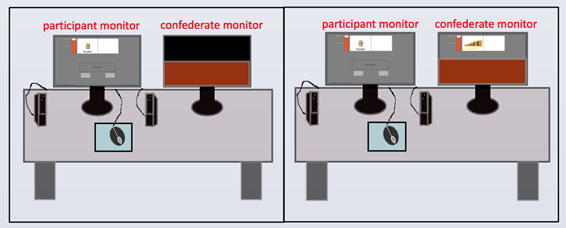
\includegraphics[width=1\linewidth]{figure2} 

}

\caption{Experimental set-up. Left, the set-up as experienced by participants in the instrumental stages of the experiment including monitors, two mini audio speakers, one mouse (with mouse mat to reduce friction). Right, the set-up as experienced by participants in the Pavlovian stage (Stage 2) of the experiment for the social conditions (see text for more explanation). The bottom half of the *confederate monitor* (in brown) covered up the response choices made by the confederate so that only stimuli and outcomes were visible to the participant but not responses.}\label{fig:figure2}
\end{figure}

\hypertarget{procedure}{%
\subsubsection{Procedure}\label{procedure}}

An example of a single trial on Stage 1 can be visualized in Figure 3.
Participants were given a pre-experiment warm-up phase to familiarize
themselves with the task during and after which questions were
permissible. Stimuli used in this warm-up phase were not used in the
experimental conditions. Conditions were controlled for order effects:
Social conditions before or after Individual conditions; DOT before or
after NonDOT conditions. Participants were not permitted to ask
questions during the experimental procedure. They were given oral
instructions before the experiment and instructions and prompts were
also provided periodically on the monitor. Participants were informed
that they would receive a cinema ticket for participation and an
additional ticket if they achieved a sufficiently high score. The entire
ToC procedure, including warm-up phase, took around 30 minutes to
complete. Following completion of the experiment (all four conditions),
participants were required to complete a questionnaire (see Appendix A).
Below is provided a description of each of the three stages of the ToC
procedure.

All stimuli (images) presented to the participants were presented
randomly, one per trial, but such that there was always an equal number
of each stimulus presented per stage.

\begin{figure}

{\centering 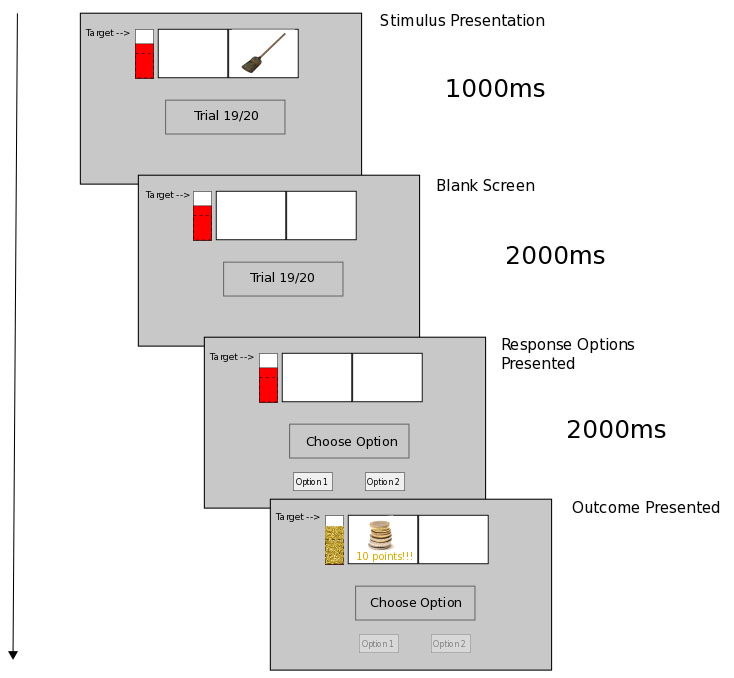
\includegraphics[width=0.6\linewidth]{figure3} 

}

\caption{Trial progression Stage 1/3. For each trial the participant was presented with a stimulus superimposed on a white panel (top right) for 1000ms, followed by a blank/white (stimulus) panel for a further 2000ms, then two response options were presented at the bottom of the screen for 2000ms. The participants were required to respond (click on one of the two options) within the 2000ms time limit or a timeout and ‘incorrect’ feedback were presented. A correct response yielded an image of money (coins) that was either small (low reward) or large (high reward) and concomitantly increased the score bar (left-side horizontal column). An incorrect response (or no response) yielded a ‘no reward’ image and a reduction of the score bar.}\label{fig:figure3}
\end{figure}

\hypertarget{stage-1-instrumental-learning-phase}{%
\subsubsection{Stage 1 -- Instrumental learning
phase:}\label{stage-1-instrumental-learning-phase}}

Twenty trials: Participants were required to learn to associate 2
different images (stimuli) with appropriate responses (click on button
option 1 or option 2) in order to get the rewarding outcome. In the DOT
condition, participants were required to associate high reward with one
stimulus (image) and low reward with the other stimulus. Incorrect
answers received a punishment (`money' loss). Participants were required
to learn to criterion here (4/5 correct responses by trial block 4): If
participants did not learn at above chance levels (2.5/5 for random
guessing) by this stage, Stage 3 (transfer of knowledge) was considered
not applicable.

\hypertarget{stage-2-pavlovian-learning-phase}{%
\subsubsection{Stage 2 -- Pavlovian learning
phase:}\label{stage-2-pavlovian-learning-phase}}

Twenty trials: Participants were required to learn to associate 4 new
images (stimuli) with rewarding outcomes. Outcomes again were comprised
of high or low reward (as in Stage 1 where the same images and audio
feedback were used for the differential outcomes). In the DOT condition
different stimuli reliably predicted high or low reward. In the NonDOT
condition different stimuli predicted reward but the reward could be
either high or low (randomly generated). In the social condition,
participants viewed a screen-capture and audio videoed performance
(confederate) on a different monitor (see Figure 2 \emph{confederate
monitor}) and were told to observe and learn from the other's
stimulus-outcome results. In the videoed performance the confederate
responded incorrectly on the first trial (met with incorrect buzzer
feedback) but responded correctly on the final 19 trials. This was the
case for both DOT and Non-DOT conditions. This approach was chosen to
increase the credibility of the confederate though it meant that the
social conditions' Stage 2 was slightly more difficult than the
individual conditions' Stage 2 (individual DOT and Non-DOT Stage 2
always provided correct stimulus-outcome pairings).

\hypertarget{stage-3-instrumental-transfer-test-phase}{%
\subsubsection{Stage 3 -- Instrumental transfer test
phase:}\label{stage-3-instrumental-transfer-test-phase}}

Twenty trials: As for Stage 1 participants again were required to
associate images (stimuli) with responses. But now it was required to
associate the 4 images used in Stage 2 to the response options in Stage
1. Note, this constituted a new set of associations for the participants
to learn.

\hypertarget{ethics}{%
\subsubsection{Ethics}\label{ethics}}

Participants were debriefed regarding their right to withdraw at any
stage of the experiment and were required to sign a consent form
regarding participation and anonymised publication of their data.

\hypertarget{results}{%
\subsection{Results}\label{results}}

The analysis carried out concerns the two (instrumental) stages for
which there were behavioural choice performance data, i.e.~Stage 1 and
Stage 3. In Stage 1 we evaluated performance (number of correct choices)
for participants in the four conditions so as to assess whether a
differential outcomes effect was obtained. In Stage 3 we evaluated
performance to assess for transfer of control (ToC).

\hypertarget{stage-1}{%
\paragraph{Stage 1}\label{stage-1}}

In Figure 4 it is shown that, as a result of overlapping error bars, no
differential outcomes effect is found in Stage 1. That is, there is no
difference in performance by the end of Stage 1 in the differential
outcomes training (DOT) versus the non-differential outcomes training
(Non-DOT) conditions in either individual or social conditions. This is
to be expected since Stage 1, based on our analysis of preceding pilot
studies, was designed to be sufficiently non-challenging so that
participants would score well above chance. Strong learning of
instrumental contingencies in Stage 1 was a prerequisite for
transferring knowledge to the test phase (Stage 3) of transfer of
control. Above chance performance by individuals on Stage 3 who show no
evidence of having learned on Stage 1 may owe to `lucky guesses'. The
absence of difference in the four conditions is desirable since
differences in performance in the test phase (Stage 3) can more
parsimoniously be attributed to learning in the Pavlovian stage (Stage
2) over conditions and the nonpossibility of categorizing new stimuli
presented in Stage 2 by common/same outcomes experienced in Stages 1 and
2.

\hypertarget{stage-3}{%
\paragraph{Stage 3}\label{stage-3}}

This instrumental stage tested the ability of participants to transfer
knowledge gained from Stage 1 (Instrumental) and Stage 2 (Pavlovian).
Differences in performance between DOT and Non-DOT conditions regarding
transfer of control are summarized in the plots in Figure 4.

\begin{figure}

{\centering 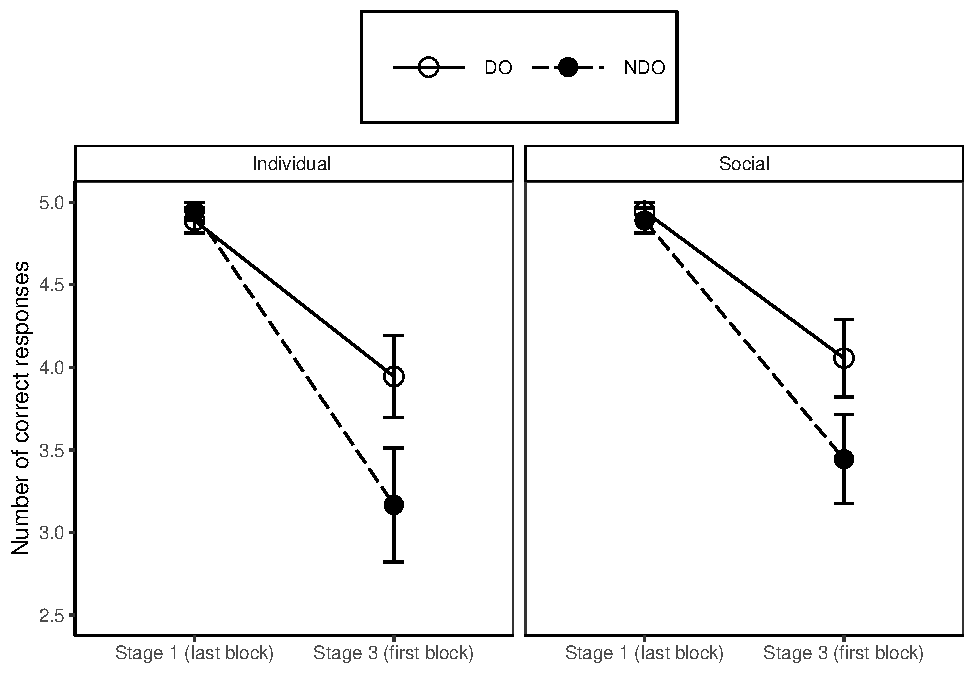
\includegraphics[width=1\linewidth]{Vicarious_value_learning_master_files/figure-latex/figure4-1} 

}

\caption{Transfer of control. Correct choice performance from the last block of trials of Stage 1 to the first block of trials in Stage 3 for non-social and social (DOT and Non-DOT) conditions. The more horizontal the line plots, the greater the transfer of control. Errorbars showing 1 SE.}\label{fig:figure4}
\end{figure}

Each block consists of 5 trials and in Stage 3 there are four different
stimuli presented. Chance performance, involving guess-work, would
produce mean scores of 2.5 (0.5 chance of getting the correct response
per trial). However, since presentation of stimuli was randomized,
participants were potentially presented several of the same stimuli
within the first block. Nevertheless, performance on the first block of
trials was considered to be the greatest indicator of transfer of
control since \emph{learning} effects (i.e.~instrumental) in subsequent
blocks (rather than direct transfer of knowledge) would be more likely
to bring to bear.

A two-way repeated measures ANOVA was run with factors: \emph{type of
outcomes} (differential versus non-differential), and \emph{type of
task} (social versus non-social). The dependent variable was amount of
correct responses (over the first block of 5 trials). A significant
effect of \emph{type of outcomes} was found, \(F\)(1, 17) = 4.991,
\(p=\) 0.039, partial \(\eta^2 =\) 0.227, with the DOT condition giving
\(M =\) 4, \(SD =\) 1.014, Non-DOT condition \(M =\) 3.306, \(SD =\)
1.305. No significant effect of \emph{type of task} was found, \(F\)(1,
17) = 0.92, \(p =\) 0.351, partial \(\eta^2 =\) 0.051. Furthermore, no
significant interaction was found \(F\)(1, 17) = 0.262, \(p =\) 0.616,
partial \(\eta^2 =\) 0.015. Two participants' data were removed for
scoring only 3/5 on the last block of stage 1, which we considered to be
at or around `chance'\footnote{See previous description of `chance'
  performance in relation to Stage 3.} performance.

\hypertarget{subjective-report}{%
\paragraph{Subjective Report}\label{subjective-report}}

Questionnaires on a 5-point Likert scale were provided to participants
to assess the extent of perceived emotional engagement in the task and
also whether they experienced the presence of the confederate
participant (social condition). Appendix A provides the results in full
for the 11 questions administered and \emph{t}-test statistical
differences from the `baseline' score of 3. One participant failed to
complete the questionnaire and so our analysis is based on 19 completed
questionnaires.

\hypertarget{discussion}{%
\subsection{Discussion}\label{discussion}}

The results presented above for Experiment 1 provide a proof of
principle that the transfer of control effect obtained when using
differential outcomes training can apply in a `social' setting and not
just the non-social setting in which it has been previously studied.
Stage 2 in the social condition served as a stage where participants
were able to learn from the video-presented stimulus-outcome pairings
(Stimulus-Expectations; S-E) of a confederate and bring to bear that
knowledge on their own outcome expectation-response (E-R) knowledge
gained from Stage 1 forming thereby the \emph{transitive bridge}
hypothesized as an explanation for individualized ToC learning. The
argument put forward by Lowe et al.
(\protect\hyperlink{ref-lowe2016minimalist}{2016}) is that participants
are able to learn from others according to a principle of
\emph{vicarious value learning}. That is, participants utilize the same
value representations (reward outcome valuations of stimuli) for others
as they do for themselves.

\hypertarget{experiment-2}{%
\section{Experiment 2}\label{experiment-2}}

\hypertarget{method-1}{%
\subsection{Method}\label{method-1}}

\hypertarget{participants-1}{%
\subsubsection{Participants}\label{participants-1}}

Thirty-three students from the University of Gothenburg participated in
each of the four conditions of Experiment 2 for the reward of a cinema
ticket. The participants were aged between 22-46 years
(\(M_{age} = 26.6\)) with 23 males and 10 females. One participant was
excluded from the EEG analysis due to highly unreliable data not
salvageable through the standardised processing steps used for all other
participants. Calculating the effect of the contrast between
differential and non-differential outcomes \emph{within} the social
level yielded Cohen's \(d=\) 0.474. Utilising this simple effect in a
sample size calculation for a one-sided t-test (directional hypothesis),
with power \(= .8\), \(\alpha = .05\), resulted in N = 29.

\hypertarget{design-1}{%
\subsubsection{Design}\label{design-1}}

The design was the same as for Study 1 with the addition of measure of
EEG. The dependent variable for the EEG activity was power spectral
density over the mu frequency band, which was extracted using fast
Fourier transform (FFT). That is amplitude in the 8-12Hz frequency
obtained from C3 and C4, which is the typical site for mu detection
since these locations are positioned over the motor cortex.
Additionally, alpha band power over the frequencies 8-12Hz for all
remaining electrodes was obtained and averaged. These were measured and
compared during the outcome presentation in Stage 2 (Pavlovian phase) in
the social and non-social conditions.

\hypertarget{materials-and-apparatus-1}{%
\subsubsection{Materials and
apparatus}\label{materials-and-apparatus-1}}

The materials were the same as for Experiment 1 with the exception of
the stimuli in the social condition and the addition of three questions
in the questionnaire as well as slight reformulations of the questions
used in Experiment 1. In Stage 2 (Pavlovian phase), the participant was
presented a video of either the face of another person (confederate)
playing the game (social condition), or an animation (non-social
condition). The function of the animation was to have a comparably
complex and informative stimulus, but that would not be social and yet
would keep participants focused during the inter-stimulus interval. The
animation consisted of a randomly moving shape where the outcome images
of Stage 1 were faded in at outcome presentation. In this way, the
non-social video provided sufficient information for the participants to
be able to perform the stimulus-outcome pairing task.

\hypertarget{objective-measure-of-confederate-emotional-expression}{%
\subsubsection{Objective measure of confederate emotional
expression}\label{objective-measure-of-confederate-emotional-expression}}

Two confederates were used to play the role of confederate during the
Pavlovian phase for the social conditions. One was used in the warm-up
stage and one in the experiment. Each confederate was instructed to
express happiness at receiving the high reward and mild frustration at
receiving low reward according to a pre-scheduled reward and cost
(punishment) schedule. As a means of assessing objectively differential
facial expressions we used the Noldus software FaceReader 8.0. Figure 5
shows this schedule for the confederate used in the experimental
condition (see Figure 6 for example expressions) over the 20 trials
(where high and low reward are generated by a random number generator in
the program and the first trial always gave a negative
reward/punishment).

\begin{figure}
\centering
\resizebox{\textwidth}{!}{
\begin{tabular}{ | c | c | c | c | c | c | c | c | c | c | c | c | c | c | c | c | c | c | c | c | c | c | }
    \hline
  \text{Stimulus Trial} & 1 & 2 & 3 & 4 & 5 & 6 & 7 & 8 & 9 & 10 & 11 & 12 & 13 & 14 & 15 & 16 & 17 & 18 & 19 & 20  \\ \hline
  \text{High Reward} &  & \cellcolor{green!25}.82 &  & \cellcolor{red!25}-.04 &  &  &  &  & \cellcolor{green!25}.10 &  & \cellcolor{green!25}.45 &\cellcolor{green!25}.39 & \cellcolor{green!25}.44 &  & \cellcolor{green!25}.18 & \cellcolor{green!25}.82 &  & \cellcolor{green!25}.36 &  & \cellcolor{green!25}.19  \\ \hline
  \text{Low Reward} &  &  & \cellcolor{red!25}-.33 &  & \cellcolor{red!25}-.41 & \cellcolor{red!25}-.24 & \cellcolor{red!25}-.20 & \cellcolor{red!25}-.28 &  & \cellcolor{red!25}-.07 &  &  &  & \cellcolor{red!25}-.29 &  &  & \cellcolor{red!25}-.16 &  & \cellcolor{red!25}-.57 &  \\ \hline
  \text{Negative Reward} & \cellcolor{red!25}-.32 &  &  &  &  &  &  &  &  &  &  &  &  &  &  &  &  &  &  &    \\
  \hline
\end{tabular}}
\caption{\textbf{FaceReader valence evaluations of confederate facial expressions in response to differential rewarding outcomes.} Valence computations were in the range -1 to 1. The table shows the maximum values recorded in response to the outcome for each trial. Key: Green-filled tabulations indicate that FaceReader computed a positive valenced expression; Red-filled tabulations indicate that FaceReader computed a negative valenced expression. All readings to 2DP.}
\label{fig:fig6}
\end{figure}

In all but one case (trial 4) the confederate expressed according to the
correct valence as computed up by FaceReader (though the negative value
in trial 4 is only slight in this case and less negative than for all
low or negative reward outcomes). An independent samples \emph{t}-test
found a significant difference between low reward (including negative
reward) vs high reward expressions, 95\% CI{[}-.86, -.43{]},
\(t(18) = -6.36\), \(p<.001\). Figure 6 shows example expressions taken
from the 20 trial sequence for positive (Figure 6 left) and negative
(Figure 6 right) valence, respectively.

\begin{figure}

{\centering 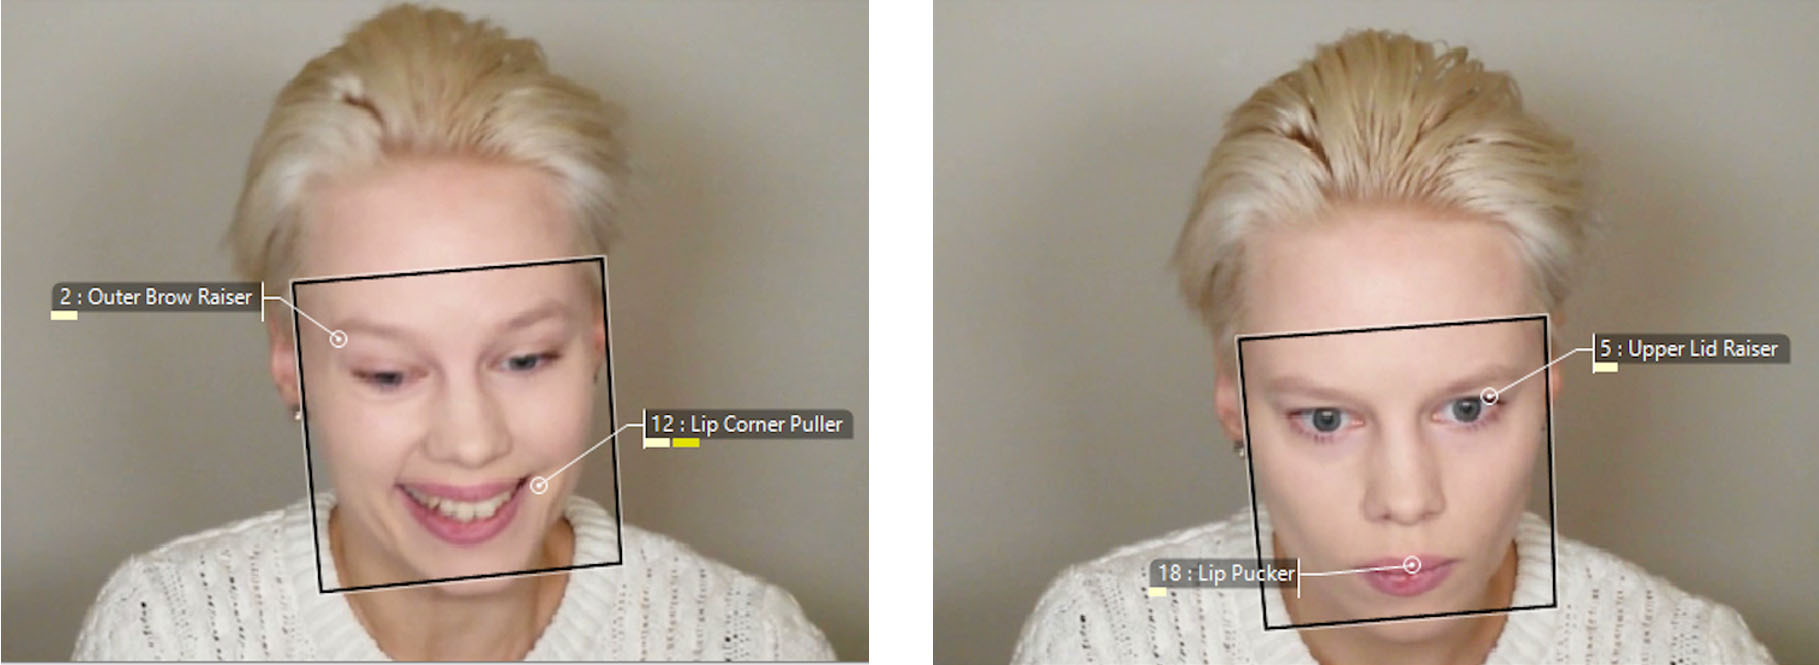
\includegraphics[width=0.8\linewidth]{figure7} 

}

\caption{FaceReader facial expression analysis visualization of confederate used in the Pavlovian social conditions. Left. The confederate expresses with positive valence. Right. The confederate expresses with negative valence. The outline box indicates the surface area over which FaceReader carries out the expression analysis. The numbered labels represent the Action Units that are expressed above baseline according to FaceReader.}\label{fig:figure6}
\end{figure}

It was observed that Action Units (see Ekman et al.,
\protect\hyperlink{ref-ekman_facial_2002}{2002}) 12, or AU12 (Lip Corner
Puller), for positively valenced expression and AU5 (Upper Lid Raiser)
for negatively valenced expression were most typically used. In the case
of the former, AU12 in the absence of expression of AU6 (cheek raiser)
may be indicative of a non-Duchenne (social) smile or that FaceReader
did not pick up all micro-expressions of the confederate. See Experiment
2 Results Discussion sub-section for more detail.

\hypertarget{electroencephalogram-recordings}{%
\subsubsection{Electroencephalogram
Recordings}\label{electroencephalogram-recordings}}

The Electroencephalogram (EEG) acquisition system OpenBCI Cyton board
was used. The Cyton board is an 8-channel neural interface, which
samples data at 250Hz. Since the present study did not analyse any
higher frequency than 25Hz, such sampling rate was deemed more than
sufficient since only a sampling rate of 2.5 times that of the frequency
is required for analysis (Cantor and Evans,
\protect\hyperlink{ref-cantor2013clinical}{2013}). The board
communicates wirelessly to a computer via Bluetooth and the data was
recorded using OpenBCI's own graphical user interface.

Further, the associated OpenBCI headset Mark IV was used. The headset is
able to target 35 electrode locations of the 10-20 system. The locations
used in Experiment 2 are those of the original locations of the headset.
After a pilot study using the device the original electrode placements
were shown to generate superior contact compared to other locations and
provided a coarse distributed signal across the scalp. Electrodes at the
earlobes were used as reference. The locations used were: Fp1, Fp2, C3,
C4, P7, P8, O1 and O2 according to the 10-20 system. Fp1, Fp2, O1 and O2
have previously been used for emotional detection (Musha et al.,
\protect\hyperlink{ref-musha1997feature}{1997}) and C3 and C4 are common
locations for detecting mu rhythmicity (Oberman et al.,
\protect\hyperlink{ref-oberman2007human}{2007}) the suppression in
activity of which (in these central brain regions) being considered to
reflect mirror neuron activity (Oberman et al.,
\protect\hyperlink{ref-oberman2007human}{2007}). It should be noted
though that the robustness of mu suppression as an indicator for mirror
neuron system activation has been questioned (Hobson and Bishop,
\protect\hyperlink{ref-hobson2016mu}{2016}).

\hypertarget{data-analysis}{%
\paragraph{Data analysis}\label{data-analysis}}

Electrodes recorded during the whole experiment but solely data from
Stage 2 when the confederate reacted to the outcomes (and the non-social
equivalent) were analysed (approximately 30 seconds per participant and
condition). To transform and interpret the EEG data, MATLAB (MathWorks,
Natick, MA, United States) and the EEGLAB toolbox (Delorme and Makeig,
\protect\hyperlink{ref-delorme2004eeglab}{2004}) were used. A
semiautomatic pipeline consisting of MATLAB-scripts imported the EEG
data alongside event markers (for events such as stimuli and outcome
presentation for the various stages), filtered it (4-45 Hz including a
notch between 48.5 and 52.5 Hz), ran independent component analysis,
removed artefacts caused by eye-blinks or power line noise spikes
(re-referenced affected channels) and extracted descriptive statistics
of the stages for each participant.

\hypertarget{procedure-1}{%
\subsubsection{Procedure}\label{procedure-1}}

The procedure used was similar to that of Experiment 1, with the
difference that participants now wore the EEG headset providing a means
to evaluate participants during the behaviourally passive Stage 2
(Pavlovian stage). Throughout the experiment, the participants were
asked to sit as still as possible without feeling unnaturally hindered
during the task. The main task-based difference between Experiment 1 and
Experiment 2 was the use of videos (visual) without audio in the
Pavlovian phase (Stage 2) of the experiment. The social video was
designed to: a) increase the sense of social presence, b) allow for
emotional expressions to provide a means for vicarious value learning
through emotional contagion. The explicit responses and outcomes of the
confederate were not shown so participants were required to make
stimulus-emotional expression associations (see Figure 7 for trial
progression) that through emotional contagion might directly tap into
the other's (stimulus) value representation. In written instructions
participants were told that they would receive points for responding
correctly, by pressing one out of two buttons on the computer screen
after a picture was presented (Stage 1). The instructions stated that
after this they would watch and observe a video relating to
simultaneously presented new pictures (Stage 2) and that they then would
perform a similar task as in Stage 1 (Stage3).

\begin{figure}

{\centering 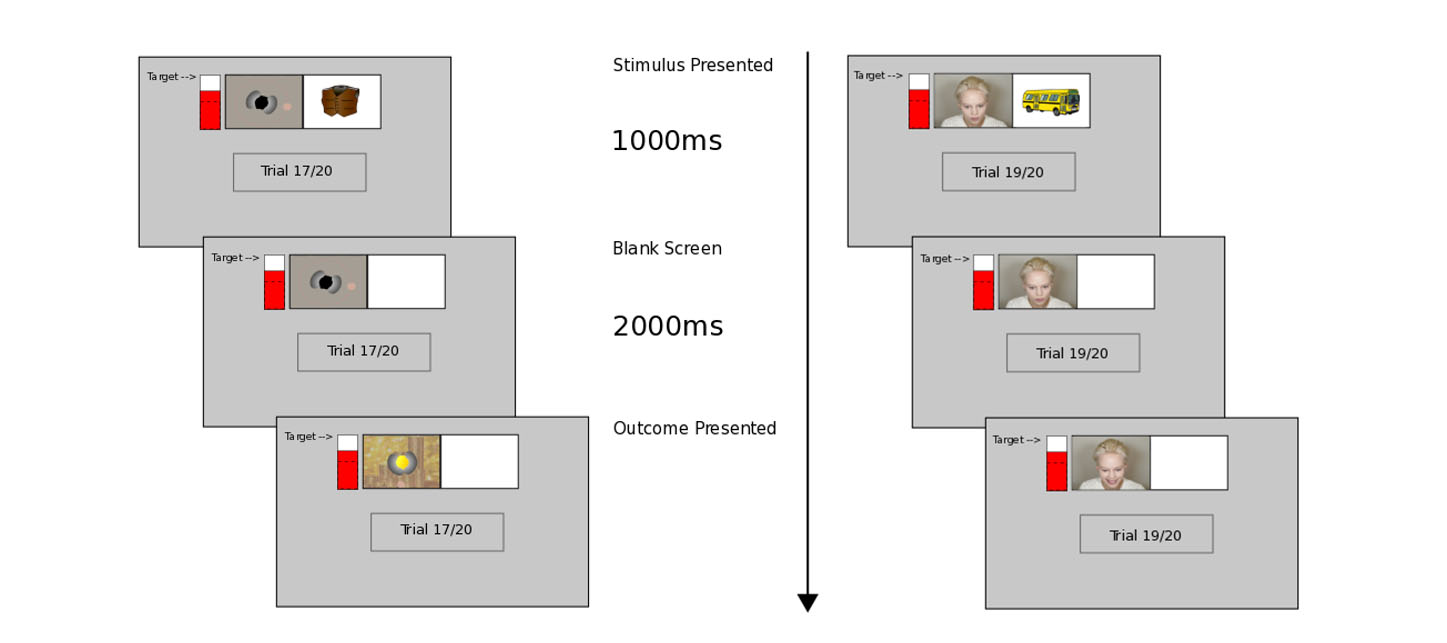
\includegraphics[width=1\linewidth]{figure8} 

}

\caption{Trial progression Stage 2. Left. Non-social animated stimulus. Right. Social video stimulus (confederate). For each trial the participant was presented with a stimulus superimposed on the right white panel (top right) for 1000ms, followed by a blank/white (stimulus) panel for a further 2000ms. The video sequence in both social and non-social conditions endured for the whole trial (left white panel). The video stimulus substituted for explicit outcomes (see Figure 3) in the social condition so that the expression of the confederate provided the only cue as to the outcomes (high reward / low reward). All but the first trial was expressed as reward – the punishment/negative reward (shocked expression), as used in Experiment 1, was intended to increase believability in the confederate. In the non-social condition outcomes were made explicit (faded in, see left bottom screen). The animation video in this non-social condition was used to control for the fact that the social condition now also used a video. The score bar (left side of screen) remained at that which the participant had achieved in Stage 1.}\label{fig:figure7}
\end{figure}

\hypertarget{ethics-1}{%
\subsubsection{Ethics}\label{ethics-1}}

The ethical considerations and procedure were as for those of Experiment
1. In addition, participants were informed prior to the study of the
uncomfortableness of the EEG headset and that they may interrupt the
study at any time.

\hypertarget{results-1}{%
\subsection{Results}\label{results-1}}

The behavioural task performance results are presented in the same way
and with the same logic as for Experiment 1, i.e.~Stage 1 and Stage 3
analyses. Stage 2 is now analysed using EEG data: comparisons of mu and
alpha band power is analysed for the social and non-social conditions.

\hypertarget{stage-1-1}{%
\subsubsection{Stage 1}\label{stage-1-1}}

Figure 8 shows, as for Experiment 1, no differential outcomes effect
(stage 1) in terms of differences in means between differential outcomes
(DOT) and non-differential outcomes (Non-DOT) conditions. As for
Experiment 1, this is desirable as we can then more reasonably attribute
in Stage 3 differences between DOT and Non-DOT in transfer of control
performance to the stages and the non-possibility of categorizing new
stimuli presented in Stage 2 by common outcomes experienced in Stages 1
and 2.

\hypertarget{stage-3-1}{%
\subsubsection{Stage 3}\label{stage-3-1}}

\begin{figure}

{\centering 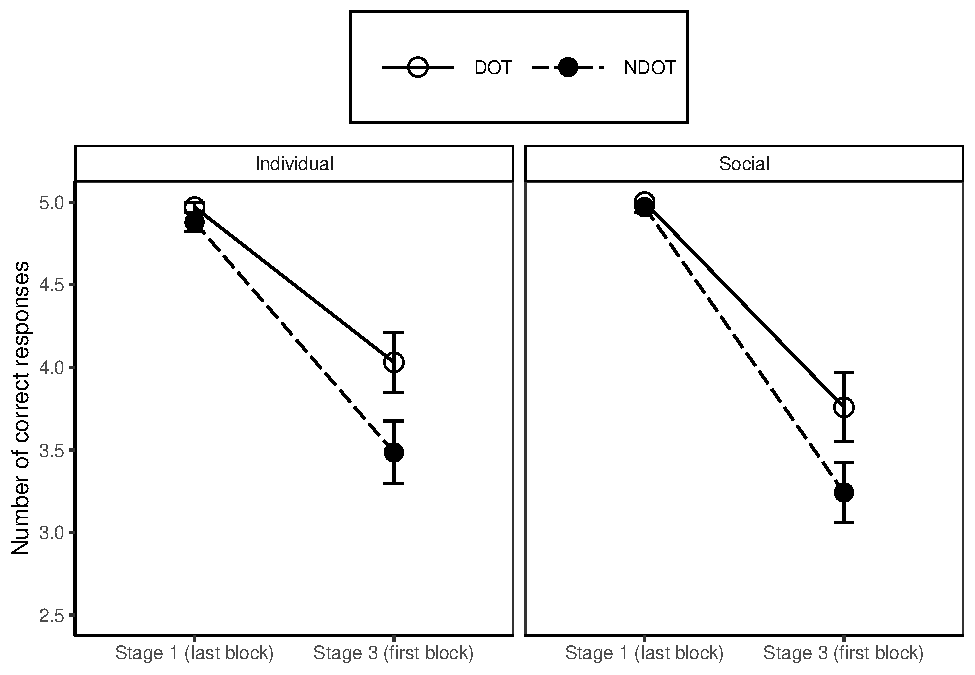
\includegraphics[width=1\linewidth]{Vicarious_value_learning_master_files/figure-latex/figure8-1} 

}

\caption{Transfer of control. Correct choice performance with errorbars from the last block of trials of Stage 1 to the first block of trials in Stage 3 for non-social and social (DOT and Non-DOT) conditions. The more horizontal the line plots, the greater the transfer of control.}\label{fig:figure8}
\end{figure}

A two-way repeated measures ANOVA was run with factors: \emph{type of
outcomes} (differential versus non-differential), and \emph{type of
task} (social versus non-social). The dependent variable was amount of
correct responses in the first 5 of 12 possible responses, in Stage 3
and differences is shown in Figure 8. A main effect of \emph{type of
outcomes} was found, \(F\)(1, 32) = 9.007, \(p=\) 0.005, partial
\(\eta^2 =\) 0.22, with the amount of correct responses being higher for
the differential outcomes (\(M =\) 3.89, \(SD =\) 1.125 correct
responses) than the non-differential outcomes (\(M =\) 3.364, \(SD =\)
1.062 correct responses). No significant effect of \emph{type of task}
was found, \(F\)(1, 32) = 1.372, \(p =\) 0.25, partial \(\eta^2 =\)
0.041 and there was no significant two-way interaction between
\emph{type of task} and \emph{type of outcomes}, \(F\)(1, 32) = 0.008,
\(p =\) 0.931, partial \(\eta^2 =\) 0.

\hypertarget{stage-2-analysis---eeg-activity}{%
\subsubsection{Stage 2 analysis - EEG
activity}\label{stage-2-analysis---eeg-activity}}

A paired-samples \emph{t}-test was used to determine whether there was a
significant mean difference in participants' mu band power between the
social and non-social videos over electrode C3 and C4. Participants
showed an unexpected increase in mu band power when observing the social
videos (\(M =\) 37.996, \(SD =\) 2.275 power spectral density) compared
to the non-social videos (\(M =\) 37.706, \(SD =\) 2.07 power spectral
density), a statistically significant mean increase of 0.29 in power
spectral density was found, 95\% CI {[}0.031, 0.548{]}, \(t\)( 31) =
2.287, \(p\) = 0.029, \(d =\) 0.404. To potentially explain this
unexpected effect three paired t-tests were used determine whether there
were significant mean amplitude differences between social and
non-social videos in the 8-12 Hz (alpha band) frequency range for
frontal, parietal and occipital electrodes. The results are shown in
table 1. Most clearly a mean difference is exhibited in the parietal
electrodes, but there also seems to be a trend towards a difference in
the occipital locations.

\begin{table}[!htbp]
\captionof{table}{Mean difference in frequency amplitude over 8-12 Hz over frontal, parietal and occipital electrodes in the social and the non-social condition.} \label{tab:title}
\centering
\begin{tabular}{lcccccccccc}
\hline
&&&& \multicolumn{2}{c}{Social} & & \multicolumn{2}{c}{Non-Social}  &  \\\cline{5-6} \cline{8-9}
&&&& Mean & SD & & Mean  & SD  & \textit{t} & \textit{p} \\
\hline
Fp1 and Fp2 &&&& 37.387  & 3.518 & & 37.154 & 3.321  & 1.486 & 0.147  \\
P7 and P8 &&&& 38.123  & 1.983 & & 37.782 & 1.777  & 2.639 & 0.013  \\
O1 and O2 &&&& 38.292  & 2.609 & & 37.997 & 2.472  & 1.903 & 0.066  \\
\hline
\\
\end{tabular}
 {\raggedright \small{\textit{Note:} SD = standard deviation. Frequency amplitude averaged over left and right electrodes.} \par}
\end{table}

\hypertarget{subjective-report-1}{%
\subsubsection{Subjective report}\label{subjective-report-1}}

Questionnaires on a 7-point Likert scale were provided to participants
to assess the extent of perceived emotional engagement in the task and
also whether they experienced the presence of the confederate
participant (social condition). Appendix B provides the results in full
for the 14 questions administered and \emph{t}-test statistical
differences from the `baseline' score of 4. Due to a relatively low
internal consistency (Cronbach's alpha = 0.674), these results are
interpreted cautiously. Admittedly it would be of interest to factorise
the items in the questionnaire and regress the number of correct
responses in Stage 3 on factor scores for ``emotional'' items. However,
due to the low internal consistency and a poor sampling adequacy
(\(KMO=\) 0.416) we could not justify such approach.

\hypertarget{discussion-1}{%
\subsection{Discussion}\label{discussion-1}}

The results indicate that, as for Experiment 1, a transfer of control
for differential outcomes based training in a social context occurs.
This conclusion is based on the significant difference in forced choice
performance in the test phase (Stage 3) of the differential outcomes
conditions versus the non-differential outcomes condition where no
interaction effect of sociality (social versus non-social conditions)
was found. In this experiment, therefore, participants appear to have
been able to learn from the affective expression of the confederate the
value of the novel stimuli and transfer this knowledge as well as that
of E-R based associations learned in Stage 1 to the test phase Stage 3.
Again, participants, at the beginning of Stage 3, have had no exposure
to the particular S-R pairings that are relevant to obtain the rewarding
outcomes.

The EEG findings, relevant for providing a measure of perceived social
presence as well as possible emotion recognition, require some
interpretation. The finding of an increase in mu band power was the
opposite of that hypothesized, however, a possible explanation for this
might be inadequate separation from posterior alpha, indicated by the
subsequent analyses of the other electrodes. The overlap between alpha
and mu have been known to generate difficulties in differentiating the
two and since attentional demand modulate alpha (Klimesch et al.,
\protect\hyperlink{ref-klimesch2007eeg}{2007}), mu suppression could be
confounded by such changes (Hobson and Bishop,
\protect\hyperlink{ref-hobson2016mu}{2016}; Oberman et al.,
\protect\hyperlink{ref-oberman2007human}{2007}). Although the conditions
were constructed and piloted as to not have differences in task
difficulty, it is possible that the individual condition required more
attention - giving rise to a suppression of alpha activity. Inescapable
differences in visual content can also have played a role. Further,
Klimesch et al. (\protect\hyperlink{ref-klimesch2007eeg}{2007}) suggests
that during observation of an action, higher level motor areas involved
in motor planning, such as the supplementary motor area (SMA), adjacent
to the pre- and primary motor cortex, should exhibit increases in mu
amplitude. It is therefore important to interpret these results in the
context of the social versus non-social conditions and what cognitive
and affective resources may have been brought to bear.

The video (social versus non-social) independent variable had no
significant effect on the amount of correct responses, also as expected.
The subjective report (questionnaire) findings also lend support to
participants either cognitively or emotionally empathizing with the
confederate. Whilst it was not explicitly asked of participants whether
they apprehended that the confederate was indeed a confederate -- for
fear of affecting future data collection -- no impressions were given by
the participants that they considered the `other' participant to be
inauthentic. Expressions of the confederates (particularly the
confederate used in Stage 2 of the Experiment, as opposed to the
training phase) did not, therefore, appear to be perceived as
`socialized' (e.g.~non-Duchenne smile) or fake.

\hypertarget{general-discussion}{%
\section{General Discussion}\label{general-discussion}}

The present article presents work aimed at evaluating whether the
differential outcomes based transfer of control effect\footnote{This
  concerns transferring knowledge from previous task stages to a third
  stage without the requirement of new learning.} (ToC) as predicted by
the Associative Two-Process theory (Trapold,
\protect\hyperlink{ref-trapold1970expectancies}{1970}; Urcuioli,
\protect\hyperlink{ref-urcuioli2005behavioral}{2005}) could apply in
social contexts. The social contextsexperimentally evaluated how a
perceived other's outcomes might be inferred: i) through direct
presentation of stimulus-outcome contingencies, ii) through indirect
presentation of outcomes as conveyed by the other's affective facial
expression. The main finding of our investigation was that the ToC
effect can apply in social contexts and was robust to the change in
contingencies (i. and ii. above) as manipulated in the two experimental
conditions reported here.

We have considered a hypothesis and explanation for this \emph{social}
ToC according to vicarious value learning (Lowe et al.,
\protect\hyperlink{ref-lowe2016minimalist}{2016}; Ruff and Fehr,
\protect\hyperlink{ref-ruff2014neurobiology}{2014}) whereby through
evaluating another's rewarding outcomes, the perceiver updates his/her
own value function -- effectively putting him/herself in the shoes of
the other. This was manipulated to occur either through direct
perception of the other's (differential) outcomes (as in Experiment 1),
or through cognitive or emotional empathizing (Drimalla et al.,
\protect\hyperlink{ref-drimalla2019face}{2019}) via affective processing
of the facial expression of other (Experiment 2). In the latter case,
facial expressions corresponded to the differential outcomes, or rather
reactions to them.

A main source of interest was to consider to what extent the
participants viewed the participating other (confederate) as being
present and as the context thereby being ``social''. In Experiment 1 and
2 we evaluated this through the use of questionnaires whereby
participant subjective reporting provided some evidence of vicarious
value learning. The Social Affective-Associative Two Process hypothesis
(Lowe et al., \protect\hyperlink{ref-lowe2016minimalist}{2016}) posits
that in non-competitive situations an individual may learn the value
function of another vicariously through emotional contagion as a result
of observing the affective expression of the other. A reinforcement
learning model was described that has been successfully deployed to
explain transfer of control (ToC) performance in individual subjects
(pigeons, rats) in non-social settings (Lowe et al.,
\protect\hyperlink{ref-lowe2017affective1}{2017}; Lowe and Billing,
\protect\hyperlink{ref-lowe2017affective}{2017}). Although the
computational model has not so far been used to model the current data
it is expected that according to the vicarious value learning
perspective it should replicate the qualitative performance of the
individual ToC. This would be the case simply because individuals are
hypothesized to use the same value function to valuate stimuli presented
to them as they would stimuli presented to the other. A ToC should not
result if a separate value function for other is represented (e.g.~in a
competitive context, see Suzuki et al.
(\protect\hyperlink{ref-suzuki2012learning}{2012}), for an example
reinforcement learning model).

The task was deliberately set up to require participants to produce fast
responses (time out and negative reward was presented for slow
responding). The aim here was to promote learning by subconscious
associative processes rather than by any other such cognitive
strategies. However, we cannot rule out that such cognitive strategies
were being used at least by a subset of the participants some of the
time. Participants may have been using a type of cognitive empathy
((Drimalla et al., \protect\hyperlink{ref-drimalla2019face}{2019}))
whereby the affective expressions of the confederate other were
evaluated and understood but not in a manner that directly tapped into
vicarious value learning (e.g.~through emotional contagion).

The uncovering of a social presence signal -- mu suppression -- as an
indicator of mirror neuron activity would have provided evidence for a
vicarious value learning strategy, however in Experiment 2 the opposite
result was found. It is suggested that this effect is a product of
inconsistent set-up of the EEG-headset and contamination from posterior
alpha, which is suggested by the subsequent follow up analysis where
parietal electrodes exhibited the same systematic amplitude difference
between conditions. However, due to the low spatial resolution of EEG it
is also difficult to differentiate between mu motor/premotor activity
and activity in other areas that are part of a larger action
observation/execution network (Oberman et al.,
\protect\hyperlink{ref-oberman2007human}{2007}). This means that if
electrodes also could pick up on activity from areas such as the SMA
(just in front of the premotor cortex). Hence, given that our electrodes
picked up mu activity from the SMA we would also see an increase in
amplitude, if the previously discussed hypothesis by Klimesch et al.
(\protect\hyperlink{ref-klimesch2007eeg}{2007}) is true. Findings from
Muthukumaraswamy and Johnson
(\protect\hyperlink{ref-muthukumaraswamy2004changes}{2004}) and
Muthukumaraswamy et al.
(\protect\hyperlink{ref-muthukumaraswamy2004mu}{2004}) do provide some
support for this claim as they recorded 8-12 Hz desynchronizations over
sensory-motor areas, and indeed, saw a synchronisation over SMA during
action observation.

We postulate, therefore, that in addition to sole contamination from
posterior alpha, the increase of mu amplitude from our electrodes at C3
and C4 could be due to synchronisation from SMA. The latter is
consistent with the possibility of suppression of egocentric activity
(self-planning) during perceived other response-outcome events. In the
present research increased amplitude in the 8-12 Hz range was found in
the social conditions as compared to the non-social (baseline)
conditions. An implication of this is that measuring synchronisation in
this range over SMA could constitute a neural signature for the
processing of social stimuli. However, further research, in combination
with simultaneous mu (de)synchronization over motor and premotor cortex
is necessary to be carried out. The presence of both would provide
stronger evidence for the existence of vicarious value learning
according to emotional contagion.

Future study is aimed at testing further the existence of vicarious
value learning through Social Affective-Associative Two Process
hypothesis, e.g.~in competitive versus noncompetitive contexts. We are
also interested in using computational models of this process for
synthetic studies, i.e.~human-robot interaction (see Lowe et al.
(\protect\hyperlink{ref-lowe2009dual}{2009}); Lowe and Ziemke
(\protect\hyperlink{ref-lowe2013exploring}{2013}); Kiryazov et al.
(\protect\hyperlink{ref-kiryazov2013role}{2013}); Alenljung et al.
(\protect\hyperlink{ref-alenljung2017user}{2017}); Andreasson et al.
(\protect\hyperlink{ref-andreasson2018affective}{2018}); Lowe et al.
(\protect\hyperlink{ref-lowe2019vicarious}{2019}); for examples) as a
further means of apprehending the validity of such affective-cognitive
processing and in the context of `minimalist' joint activity (or joint
action) research (Vesper et al.,
\protect\hyperlink{ref-vesper2010minimal}{2010}), which focuses on the
use of associative mechanisms to produce intelligent collaborative
behaviour.

\hypertarget{competing-interests-statement}{%
\section{Competing Interests
Statement}\label{competing-interests-statement}}

The authors are not aware of any competing interests that publication of
this article would result in.

\hypertarget{informed-consent}{%
\section{Informed consent}\label{informed-consent}}

All human participants were informed of their right to withdraw from the
experiments at any time and gave approval to our right to publish
(anonymously) their data. The actress (confederate) used in experiment 2
also gave written consent for us to use images of her.

\hypertarget{references}{%
\section*{References}\label{references}}
\addcontentsline{toc}{section}{References}

\begingroup
\setlength{\parindent}{-0.5in}
\setlength{\leftskip}{0.5in}

\hypertarget{refs}{}
\leavevmode\hypertarget{ref-addison_examination_2006}{}%
Addison, L., 2006. An examination of the differential outcomes effect
when teaching discriminations to children with autism and other
developmental disabilities. ProQuest Dissertations Publishing.

\leavevmode\hypertarget{ref-adelmann1989facial}{}%
Adelmann, P.K., Zajonc, R.B., 1989. Facial efference and the experience
of emotion. Annual review of psychology 40, 249--280.

\leavevmode\hypertarget{ref-alenljung2017user}{}%
Alenljung, B., Andreasson, R., Billing, E.A., Lindblom, J., Lowe, R.,
2017. User experience of conveying emotions by touch, in: 2017 26th Ieee
International Symposium on Robot and Human Interactive Communication
(Ro-Man). IEEE, pp. 1240--1247.

\leavevmode\hypertarget{ref-andreasson2018affective}{}%
Andreasson, R., Alenljung, B., Billing, E., Lowe, R., 2018. Affective
touch in human--robot interaction: Conveying emotion to the nao robot.
International Journal of Social Robotics 10, 473--491.

\leavevmode\hypertarget{ref-baron2004empathy}{}%
Baron-Cohen, S., Wheelwright, S., 2004. The empathy quotient: An
investigation of adults with asperger syndrome or high functioning
autism, and normal sex differences. Journal of autism and developmental
disorders 34, 163--175.

\leavevmode\hypertarget{ref-bradley2007international}{}%
Bradley, M.M., Lang, P.J., 2007. The international affective digitized
sounds (; iads-2): Affective ratings of sounds and instruction manual.
University of Florida, Gainesville, FL, Tech. Rep. B-3.

\leavevmode\hypertarget{ref-cantor2013clinical}{}%
Cantor, D.S., Evans, J.R., 2013. Clinical neurotherapy: Application of
techniques for treatment. Academic Press.

\leavevmode\hypertarget{ref-carmona2019differential}{}%
Carmona, I., Vivas, A.B., Estévez, A.F., 2019. Differential outcomes
training ameliorates visual memory impairments in patients with
alzheimer's disease: A pilot study. Frontiers in psychology 9, 2671.

\leavevmode\hypertarget{ref-delorme2004eeglab}{}%
Delorme, A., Makeig, S., 2004. EEGLAB: An open source toolbox for
analysis of single-trial eeg dynamics including independent component
analysis. Journal of neuroscience methods 134, 9--21.

\leavevmode\hypertarget{ref-drimalla2019face}{}%
Drimalla, H., Landwehr, N., Hess, U., Dziobek, I., 2019. From face to
face: The contribution of facial mimicry to cognitive and emotional
empathy. Cognition and Emotion 33, 1672--1686.

\leavevmode\hypertarget{ref-dziobek2011neuronal}{}%
Dziobek, I., Preißler, S., Grozdanovic, Z., Heuser, I., Heekeren, H.R.,
Roepke, S., 2011. Neuronal correlates of altered empathy and social
cognition in borderline personality disorder. Neuroimage 57, 539--548.

\leavevmode\hypertarget{ref-ekman_facial_2002}{}%
Ekman, P., Hager, J.C., Friesen, W.V., 2002. Facial action coding system
: The manual. Research Nexus, Salt Lake City.

\leavevmode\hypertarget{ref-enticott2008mirror}{}%
Enticott, P.G., Johnston, P.J., Herring, S.E., Hoy, K.E., Fitzgerald,
P.B., 2008. Mirror neuron activation is associated with facial emotion
processing. Neuropsychologia 46, 2851--2854.

\leavevmode\hypertarget{ref-esteban2014differential}{}%
Esteban, L., Plaza, V., López-Crespo, G., Vivas, A.B., Estévez, A.F.,
2014. Differential outcomes training improves face recognition memory in
children and in adults with down syndrome. Research in developmental
disabilities 35, 1384--1392.

\leavevmode\hypertarget{ref-estevez2001differential}{}%
Estévez, A.F., Fuentes, L.J., Marı-Bêffa, P., González, C., Alvarez, D.,
2001. The differential outcome effect as a useful tool to improve
conditional discrimination learning in children. Learning and Motivation
32, 48--64.

\leavevmode\hypertarget{ref-estevez2003differential}{}%
Estévez, A.F., Fuentes, L.J., Overmier, J.B., González, C., 2003.
Differential outcomes effect in children and adults with down syndrome.
American Journal on Mental Retardation 108, 108--116.

\leavevmode\hypertarget{ref-faul2007g}{}%
Faul, F., Erdfelder, E., Lang, A.-G., Buchner, A., 2007. G* power 3: A
flexible statistical power analysis program for the social, behavioral,
and biomedical sciences. Behavior research methods 39, 175--191.

\leavevmode\hypertarget{ref-hall2003acquired}{}%
Hall, G., Mitchell, C., Graham, S., Lavis, Y., 2003. Acquired
equivalence and distinctiveness in human discrimination learning:
Evidence for associative mediation. Journal of Experimental Psychology:
General 132, 266.

\leavevmode\hypertarget{ref-hatfield1993emotional}{}%
Hatfield, E., Cacioppo, J.T., Rapson, R.L., 1993. Emotional contagion.
Current directions in psychological science 2, 96--100.

\leavevmode\hypertarget{ref-hess2013emotional}{}%
Hess, U., Fischer, A., 2013. Emotional mimicry as social regulation.
Personality and social psychology review 17, 142--157.

\leavevmode\hypertarget{ref-hobson2016mu}{}%
Hobson, H.M., Bishop, D.V., 2016. Mu suppression--a good measure of the
human mirror neuron system? cortex 82, 290--310.

\leavevmode\hypertarget{ref-kiryazov2013role}{}%
Kiryazov, K., Lowe, R., Becker-Asano, C., Randazzo, M., 2013. The role
of arousal in two-resource problem tasks for humanoid service robots,
in: 2013 Ieee Ro-Man. IEEE, pp. 62--69.

\leavevmode\hypertarget{ref-klimesch2007eeg}{}%
Klimesch, W., Sauseng, P., Hanslmayr, S., 2007. EEG alpha oscillations:
The inhibition--timing hypothesis. Brain research reviews 53, 63--88.

\leavevmode\hypertarget{ref-lowe2017affective1}{}%
Lowe, R., Almér, A., Billing, E., Sandamirskaya, Y., Balkenius, C.,
2017. Affective--associative two-process theory: A neurocomputational
account of partial reinforcement extinction effects. Biological
cybernetics 111, 365--388.

\leavevmode\hypertarget{ref-lowe2019vicarious}{}%
Lowe, R., Almér, A., Gander, P., Balkenius, C., 2019. Vicarious value
learning and inference in human-human and human-robot interaction, in:
2019 8th International Conference on Affective Computing and Intelligent
Interaction Workshops and Demos (Aciiw). IEEE, pp. 395--400.

\leavevmode\hypertarget{ref-lowe2016minimalist}{}%
Lowe, R., Almér, A., Lindblad, G., Gander, P., Michael, J., Vesper, C.,
2016. Minimalist social-affective value for use in joint action: A
neural-computational hypothesis. Frontiers in computational neuroscience
10, 88.

\leavevmode\hypertarget{ref-lowe2017affective}{}%
Lowe, R., Billing, E., 2017. Affective-associative two-process theory: A
neural network investigation of adaptive behaviour in differential
outcomes training. Adaptive Behavior 25, 5--23.

\leavevmode\hypertarget{ref-lowe2009dual}{}%
Lowe, R., Humphries, M., Ziemke, T., 2009. The dual-route hypothesis:
Evaluating a neurocomputational model of fear conditioning in rats.
Connection Science 21, 15--37.

\leavevmode\hypertarget{ref-lowe2014neural}{}%
Lowe, R., Sandamirskaya, Y., Billing, E., 2014. A neural dynamic model
of associative two-process theory: The differential outcomes effect and
infant development, in: 4th International Conference on Development and
Learning and on Epigenetic Robotics. IEEE, pp. 440--447.

\leavevmode\hypertarget{ref-lowe2013exploring}{}%
Lowe, R., Ziemke, T., 2013. Exploring the relationship of reward and
punishment in reinforcement learning, in: 2013 Ieee Symposium on
Adaptive Dynamic Programming and Reinforcement Learning (Adprl). IEEE,
pp. 140--147.

\leavevmode\hypertarget{ref-maki1995expectancies}{}%
Maki, P., Overmier, J.B., Delos, S., Gutmann, A.J., 1995. Expectancies
as factors influencing conditional discrimination performance of
children. The Psychological Record 45, 45--72.

\leavevmode\hypertarget{ref-martinez2013effects}{}%
Martı́nez, L., Flores, P., González-Salinas, C., Fuentes, L.J., Estévez,
A.F., 2013. The effects of differential outcomes and different types of
consequential stimuli on 7-year-old children's discriminative learning
and memory. Learning \& behavior 41, 298--308.

\leavevmode\hypertarget{ref-mccormack2017differential}{}%
McCormack, J., Arnold-Saritepe, A., Elliffe, D., 2017. The differential
outcomes effect in children with autism. Behavioral Interventions 32,
357--369.

\leavevmode\hypertarget{ref-mccormack2019quantifying}{}%
McCormack, J.C., Elliffe, D., Virués-Ortega, J., 2019. Quantifying the
effects of the differential outcomes procedure in humans: A systematic
review and a meta-analysis. Journal of applied behavior analysis 52,
870--892.

\leavevmode\hypertarget{ref-meehan1999class}{}%
Meehan, E.F., 1999. Class-consistent differential reinforcement and
stimulus class formation in pigeons. Journal of the Experimental
Analysis of Behavior 72, 97--115.

\leavevmode\hypertarget{ref-miller2002differential}{}%
Miller, O.T., Waugh, K.M., Chambers, K., 2002. Differential outcomes
effect: Increased accuracy in adults learning kanji with stimulus
specific rewards. The Psychological Record 52, 315--324.

\leavevmode\hypertarget{ref-mok2009neural}{}%
Mok, L.W., Thomas, K.M., Lungu, O.V., Overmier, J.B., 2009. Neural
correlates of cue-unique outcome expectations under differential
outcomes training: An fMRI study. Brain Research 1265, 111--127.

\leavevmode\hypertarget{ref-molina2015differential}{}%
Molina, M., Plaza, V., Fuentes, L.J., Estévez, A.F., 2015. The
differential outcomes procedure enhances adherence to treatment: A
simulated study with healthy adults. Frontiers in psychology 6, 1780.

\leavevmode\hypertarget{ref-MOORE2012309}{}%
Moore, A., Gorodnitsky, I., Pineda, J., 2012. EEG mu component responses
to viewing emotional faces. Behavioural Brain Research 226, 309--316.
doi:\href{https://doi.org/https://doi.org/10.1016/j.bbr.2011.07.048}{https://doi.org/10.1016/j.bbr.2011.07.048}

\leavevmode\hypertarget{ref-MooreMatthew2017Mrsi}{}%
Moore, M., Franz, E., 2017. Mu rhythm suppression is associated with the
classification of emotion in faces. Cognitive, Affective, \& Behavioral
Neuroscience 17, 224--234.

\leavevmode\hypertarget{ref-musha1997feature}{}%
Musha, T., Terasaki, Y., Haque, H.A., Ivamitsky, G.A., 1997. Feature
extraction from eegs associated with emotions. Artificial Life and
Robotics 1, 15--19.

\leavevmode\hypertarget{ref-muthukumaraswamy2004changes}{}%
Muthukumaraswamy, S.D., Johnson, B., 2004. Changes in rolandic mu rhythm
during observation of a precision grip. Psychophysiology 41, 152--156.

\leavevmode\hypertarget{ref-muthukumaraswamy2004mu}{}%
Muthukumaraswamy, S.D., Johnson, B.W., McNair, N.A., 2004. Mu rhythm
modulation during observation of an object-directed grasp. Cognitive
brain research 19, 195--201.

\leavevmode\hypertarget{ref-oberman2007human}{}%
Oberman, L.M., Pineda, J.A., Ramachandran, V.S., 2007. The human mirror
neuron system: A link between action observation and social skills.
Social cognitive and affective neuroscience 2, 62--66.

\leavevmode\hypertarget{ref-peterson1980effects}{}%
Peterson, G.B., Trapold, M.A., 1980. Effects of altering outcome
expectancies on pigeons' delayed conditional discrimination performance.
Learning and Motivation 11, 267--288.

\leavevmode\hypertarget{ref-PinedaJaimeA2005Tfso}{}%
Pineda, J.A., 2005. The functional significance of mu rhythms:
Translating "seeing" and "hearing" into "doing". Brain Research Reviews
50, 57--68.

\leavevmode\hypertarget{ref-plaza2012improving}{}%
Plaza, V., López-Crespo, G., Antúnez, C., Fuentes, L.J., Estévez, A.F.,
2012. Improving delayed face recognition in alzheimer's disease by
differential outcomes. Neuropsychology 26, 483.

\leavevmode\hypertarget{ref-plaza2018learning}{}%
Plaza, V., Molina, M., Fuentes, L.J., Estévez, A.F., 2018. Learning and
recall of medical treatment-related information in older adults using
the differential outcomes procedure. Frontiers in psychology 9, 157.

\leavevmode\hypertarget{ref-GiacomoRizzolatti2001Nmut}{}%
Rizzolatti, G., Fogassi, L., Gallese, V., 2001. Neurophysiological
mechanisms underlying the understanding and imitation of action. Nature
Reviews Neuroscience 2, 661.

\leavevmode\hypertarget{ref-ruff2014neurobiology}{}%
Ruff, C.C., Fehr, E., 2014. The neurobiology of rewards and values in
social decision making. Nature Reviews Neuroscience 15, 549--562.

\leavevmode\hypertarget{ref-singer2009social}{}%
Singer, T., Lamm, C., 2009. The social neuroscience of empathy. Annals
of the New York Academy of Sciences 1156, 81--96.

\leavevmode\hypertarget{ref-snodgrass1980standardized}{}%
Snodgrass, J.G., Vanderwart, M., 1980. A standardized set of 260
pictures: Norms for name agreement, image agreement, familiarity, and
visual complexity. Journal of experimental psychology: Human learning
and memory 6, 174.

\leavevmode\hypertarget{ref-suzuki2012learning}{}%
Suzuki, S., Harasawa, N., Ueno, K., Gardner, J.L., Ichinohe, N., Haruno,
M., Cheng, K., Nakahara, H., 2012. Learning to simulate others'
decisions. Neuron 74, 1125--1137.

\leavevmode\hypertarget{ref-trapold1970expectancies}{}%
Trapold, M.A., 1970. Are expectancies based upon different positive
reinforcing events discriminably different? Learning and Motivation 1,
129--140.

\leavevmode\hypertarget{ref-urcuioli2005behavioral}{}%
Urcuioli, P.J., 2005. Behavioral and associative effects of differential
outcomes in discrimination learning. Animal Learning \& Behavior 33,
1--21.

\leavevmode\hypertarget{ref-vesper2010minimal}{}%
Vesper, C., Butterfill, S., Knoblich, G., Sebanz, N., 2010. A minimal
architecture for joint action. Neural Networks 23, 998--1003.

\leavevmode\hypertarget{ref-wicker2003both}{}%
Wicker, B., Keysers, C., Plailly, J., Royet, J.-P., Gallese, V.,
Rizzolatti, G., 2003. Both of us disgusted in my insula: The common
neural basis of seeing and feeling disgust. Neuron 40, 655--664.

\endgroup

\hypertarget{appendix}{%
\section{Appendix}\label{appendix}}

\hypertarget{a}{%
\subsection{A}\label{a}}

Questionnaire for experiment 1.

\begin{figure}
\centering
\resizebox{\textwidth}{!}{
\begin{tabular}{|l|l|l|l|l|l|}
\hline & \text { Question } & M & \text { Md } & S D & \text { Different from 3 } \\
\hline 
\text { Q1 } & \text { Iunderstood which options were the most rewarding } & 4 & 4 & 0.882 &\cellcolor{orange!15}t(18)=4.943, p<.001 \\
\hline 
\text { Q2 } & \text { I found the game engaging } & 3.63 & 4 & 0.761 &\cellcolor{orange!15}t(18)=3.618, p=.002  \\
\hline 
\text { Q3 } & \text { I experienced anxiety while playing the game } & 2.58 & 2 & 1.121 & t(18)=-1.637, p=.119 \\
\hline 
\text { Q4 } & \text { I experienced fustration while playing the game } & 2.74 & 3 & 1.327 &  t(18) =0.865, p=.399 \\
\hline 
\text { Q5 } & \text { I experienced excitement while playing the game } & 3.58 & 4 & 0.769 &\cellcolor{orange!15}t(18) =3.284, p=.004 \\
\hline 
\text { Q6 } & \text { I experienced happiness while playing the game } & 3.26 & 3 & 0.806 &  t(18)=1.424, p=.172  \\
\hline 
\text { Q7 } & \text { I experienced that the other person participated in the activity } & 3.53 & 4 & 1.219 &  t(18)=1.882, p=.076 \\
\hline 
\text { Q8 } & \text { I understood what the other person was doing } & 3.53 & 4 & 1.264 & t(18)=1.816, p=.086 \\
\hline 
\text { Q9 } & \text { I experienced the other person's goals } & 3.74 & 4 & 1.240 &\cellcolor{orange!15}t(18)=2.590, p=.018 \\
\hline
\text { Q10 } & \text { I knew what the other person felt } & 2.89 & 3 & 1.1 & t(18)=0.417, p=.682 \\
\hline 
\text { Q11 } & \text { I experienced the other person's emotions } & 2.53 & 3 & 1.124 & t(18)=1.837, p=.083 \\
\hline
\end{tabular}}\end{figure}

\hypertarget{b}{%
\subsection{B}\label{b}}

Questionnaire for experiment 2. As in Study 1, a post-study
questionnaire was used. Questions 1 to 11 were improved by slight
reformulations and three additional questions were added (see Appendix
A). The answering scale used was a 7-point Likert scale.

\begin{figure}
\centering
\resizebox{\textwidth}{!}{
\begin{tabular}{|l|l|l|l|l|l|}
\hline 
& Question & M & Md & SD & Different from 4  \\
&  &  &  &  & (bonferroni adjusted) \\
\hline 
Q1 & I understood which options were the most rewarding & 4.79 & 5 & 1.364 &\cellcolor{orange!15}t(32)=3.319, p=.032 \\
\hline 
Q2 & I found the task engaging & 5.27 & 6 & 1.376 &\cellcolor{orange!15}t(32)=5.315, p<.001 \\
\hline 
Q3 & Iexperienced anxiety while performing the task & 3.15 & 3 & 1.752 & t(32)=2.782, p=1.00 \\
\hline 
Q4 & I experienced frustration while performing the task & 3.7 & 4 & 1.811 & t(32)=0.961, p=1.00 \\
\hline 
Q5 & I experienced exciterment while performing the task & 5 & 5 & 1.346 &\cellcolor{orange!15}t(32)=4.267, p=.002 \\
\hline 
Q6 & I experienced happiness while performing the task & 4.48 & 5 & 1.439 & t(32)=1.9366, p=.865 \\
\hline 
Q7 & I experienced that the other participant was involved in the activity & 4.61 & 5 & 1.936 & t(32)=1.799, p=1.00 \\
\hline 
Q8 & I understood what the other participant was doing & 4.3 & 4 & 1.667 & t(32)=1.044, p=1.00 \\
\hline 
Q9 & I did not experience the other participant's goals & 3.73 & 4 & 1.547 & t(32)=1.0449, p=1.00 \\
\hline 
Q10 & I recognized what the other participant felt & 5.61 & 6 & 1.116 &\cellcolor{orange!15}t(32)=8.265, p<.001 \\
\hline 
Q11 & I experienced the other participant's emotions & 5.12 & 5 & 1.516 &\cellcolor{orange!15}t(32)=4.249, p=0.02 \\
\hline 
Q12 & I did not experience the animation as an active agent & 5.27 & 5 & 1.719 &\cellcolor{orange!15}t(32)-4.554, p=.002 \\
\hline 
Q13 & I could draw the connections between what occurred in the animation and the pictures presented & 3.21 & 2 & 2.027 &  t(32)=-2.233, p=1.00 \\  
\hline 
Q14 & I could draw the connections between the other participant's reactions and the pictures presented & 4.09 & 4 & 1.792 & t(32)=0.291, p=1.00   \\
\hline
\end{tabular}}
\end{figure}


\end{document}


